\documentclass[12pt]{article}

\usepackage{amsmath}
\usepackage{graphicx}
\usepackage[margin=1in]{geometry}
\usepackage[style=authoryear,backend=biber]{biblatex}
\addbibresource{impact.bib}

\begin{document}
\title{Foreign Buyer Revisionism}

\section{Introduction}

Taxes and restrictions on foreign purchases of residences have been implemented in multiple jurisdictions worldwide with the stated purpose of making homes more affordable for domestic residents. For example, in extending a ban on foreign purchases of Canadian residential real estate, a government press release stated: ``For years, foreign money has been coming into Canada to buy up residential real estate, increasing housing affordability concerns in cities across the country, and particularly in major urban centres. Foreign ownership has also fueled worries about Canadians being priced out of housing markets in cities and towns across the country.''\footnote{\textcite{gOC}.}

There are theoretical and empirical reasons to expect foreign buyer taxes to
succeed in bringing down local housing prices, many of which are detailed in a
comprehensive study by \textcite{favilukisVanNieuwerburgh}. The disincentive to
purchase homes should reduce the pool of buyers and lower willigness to pay
among remaining foreign buyers. This reduction in prices hurts landlords and
incumbent property owners through lost property value and rents, but makes
homes more affordable for renters. There may be an associated loss of
construction jobs, and the analysis in \textcite{favilukisVanNieuwerburgh} does
not consider the effect of reciprocal taxes on domestic residents who may wish
to purchase property overseas.\footnote{It is not obvious that a target country
would wish to reciprocate to disincentivize the host country's tax. For
example, China, the source of most foreign buying in Canada prior to the recent
spate of taxes (per \textcite{ctvNews}) has made efforts to discourage capital
flight.}

Existing studies of the impact of the entry and exit of foreign buyers on local
home prices are mixed, with some finding large effects in the predicted
direction, as summarized in \textcite{davidoffZheng}. \textcite{LiShenZhang},
\textcite{gorbackGlobalCapitalLocal2020}, \textcite{pavlovImmigrationFlows},
and \textcite{BadarinzaRamadorai} find that within metropolitan areas,
submarkets exposed to foreign buyers see larger price increases when the types
of foreign buyers prone to buy in those submarkets face increased incentives to
buy overseas. \textcite{DachisDurantonTurner}, \textcite{klevenBest},
\textcite{kopczukMunroe}, and \textcite{davidoffLeigh} find, as a general
matter, that increasing transaction taxes on housing purchases leads to fewer
transactions and lower prices. \textcite{HartleyForeign},
\textcite{andalfattoEstimatingEffectMetro2023}, \textcite{DuYinZhang}, and
\textcite{pavlovForeignBuyerTaxes} collectively find that foreign buyer taxes
in Australia, Canada, and New Zealand led to lower prices.

As \textcite{favilukisVanNieuwerburgh} observe, foreign buyers may not leave
homes empty, but rather rent them out to locals. In their calibration, this
changes the social welfare effect of foreign buyers from negative to slightly
positive. The effect of out of town buyers is moderate because local investors
are so price sensitive in their demand for rental properties and out-of-town
buyers represent a small share of overall capital investment. In this way,
foreign buyers represent a slightly positive form of capital accumulation. This
is a relevant case, as British Columbia has imposed significant taxes on empty
homes and vacation properties in urban areas while also imposing significant
taxes on foreign buyers, and the Canadian federal government has both imposed
taxes on empty homes owned by foreigners and has temporarily banned the
purchase of single residences by foreigners.

At the time of writing, construction in Canadian cities, particularly
condominiums in the most expensive cities, Vancouver and Toronto, has slowed
dramatically. This has led some observers to suggest that the taxation of
foreign buyers has overshot, leading to a negative supply response larger than
the positive demand response on prices from foreign buying, such that locals
have been adversely affected. It is thus worthwhile asking whether there is
empirical evidence supporting the idea that foreign buyers, particularly in the
presence of empty homes taxes, may have positive welfare effects and their
taxation adverse effects on housing affordability for locals.

There are several channels through which foreign buyers could have positive
affordability effects. First, per \textcite{favilukisVanNieuwerburgh}, foreign
buyers may rent houses to locals, particularly in the presence of an empty
homes tax. 

Second, foreign buyers may purchase condominiums in the presale phase of
condominium development and then assign their contracts prior to completion.
The presence of foreign presale purchasers would raise presale prices,
encouraging the supply of condominiums, but with no increase in demand for
occupied space. The net effect of that form of investment should be positive
for affordability, with an adverse competition effect for locals who wish to
occupy homes purchased through the presale channel.

A third possibility is that foreign buyers could have a beneficial effect on
housing affordability for most locals if they have a relative preference for
quality, and if there is a high degree of vertical differentiation within
buildings. To see this channel, consider a limiting case in which top-floor
penthouse units have a high level of quality, and all homes below the penthouse
have a lower level of quality. For simplicity, assume all buildings are 10
storeys tall. If steady state, construction supply is infinitely elastic at a
price of \$X, then if foreign investors are permitted in a market, then the
price to locals will be:

\begin{align}
	.9p_{l}(q) + .1p_{f} = X\\
	p_{l} = \frac{X - .1p_{f}}{.9}.
\end{align}

Without foreign buyers, the price of lower-quality units would be $p_{l} =
\frac{X-.1p_{d}}{.9}$. In that way, luxury foreign demand could crowd out local
luxury demand, but subsidize local consumption of generic units.

\section{Do foreign buyers leave homes empty?}

Per \textcite{specTax2019}, of 3,709 foreign owners deemed subject
to the empty homes tax in 2018, 1,205 transitioned to renting their homes out
in 2019, 1,413 sold their property, 951 remained subject to the tax, and only
66 transitioned to primary residence. 

\section{Do foreign buyers specialize in the most luxurious units within buildings?}

Figure \ref{fig:variance_decomposition} presents suggestive evidence on the question of
whether foreign buyers may offer implicit subsidies to local buyers of
standard-quality units through abnormally high willingness to pay for higher
quality units, for example, those with prime views. The data are taken from
condominium resales in Greater Vancouver between 2010 and 2023, with data
provided by BC Assessment. The plot measures the year of transactions on the
horizontal axis. On the vertical axis are measures of the variance of the
natural logarithm of transaction prices by year. The red line plots the
variance of all transaction prices. The green plots the variance of mean prices
across buildings.\footnote{If there were only one transaction for each building
with a transaction in a given year, the red and green lines would coincide.}
The blue line plots the mean variance of log transaction prices within
buildings. 

The dashed vertical line in Figure \ref{fig:variance_decomposition} coincides
with the imposition of the foreign buyer tax in July, 2016. Consistent with
foreign buyers demanding more expensive units [CITE], the overall variance of
prices drops sharply in the years after the tax, consistent with loss of an important luxury
segment of the market. However, the reduction in price variance appears to be
almost entirely driven by

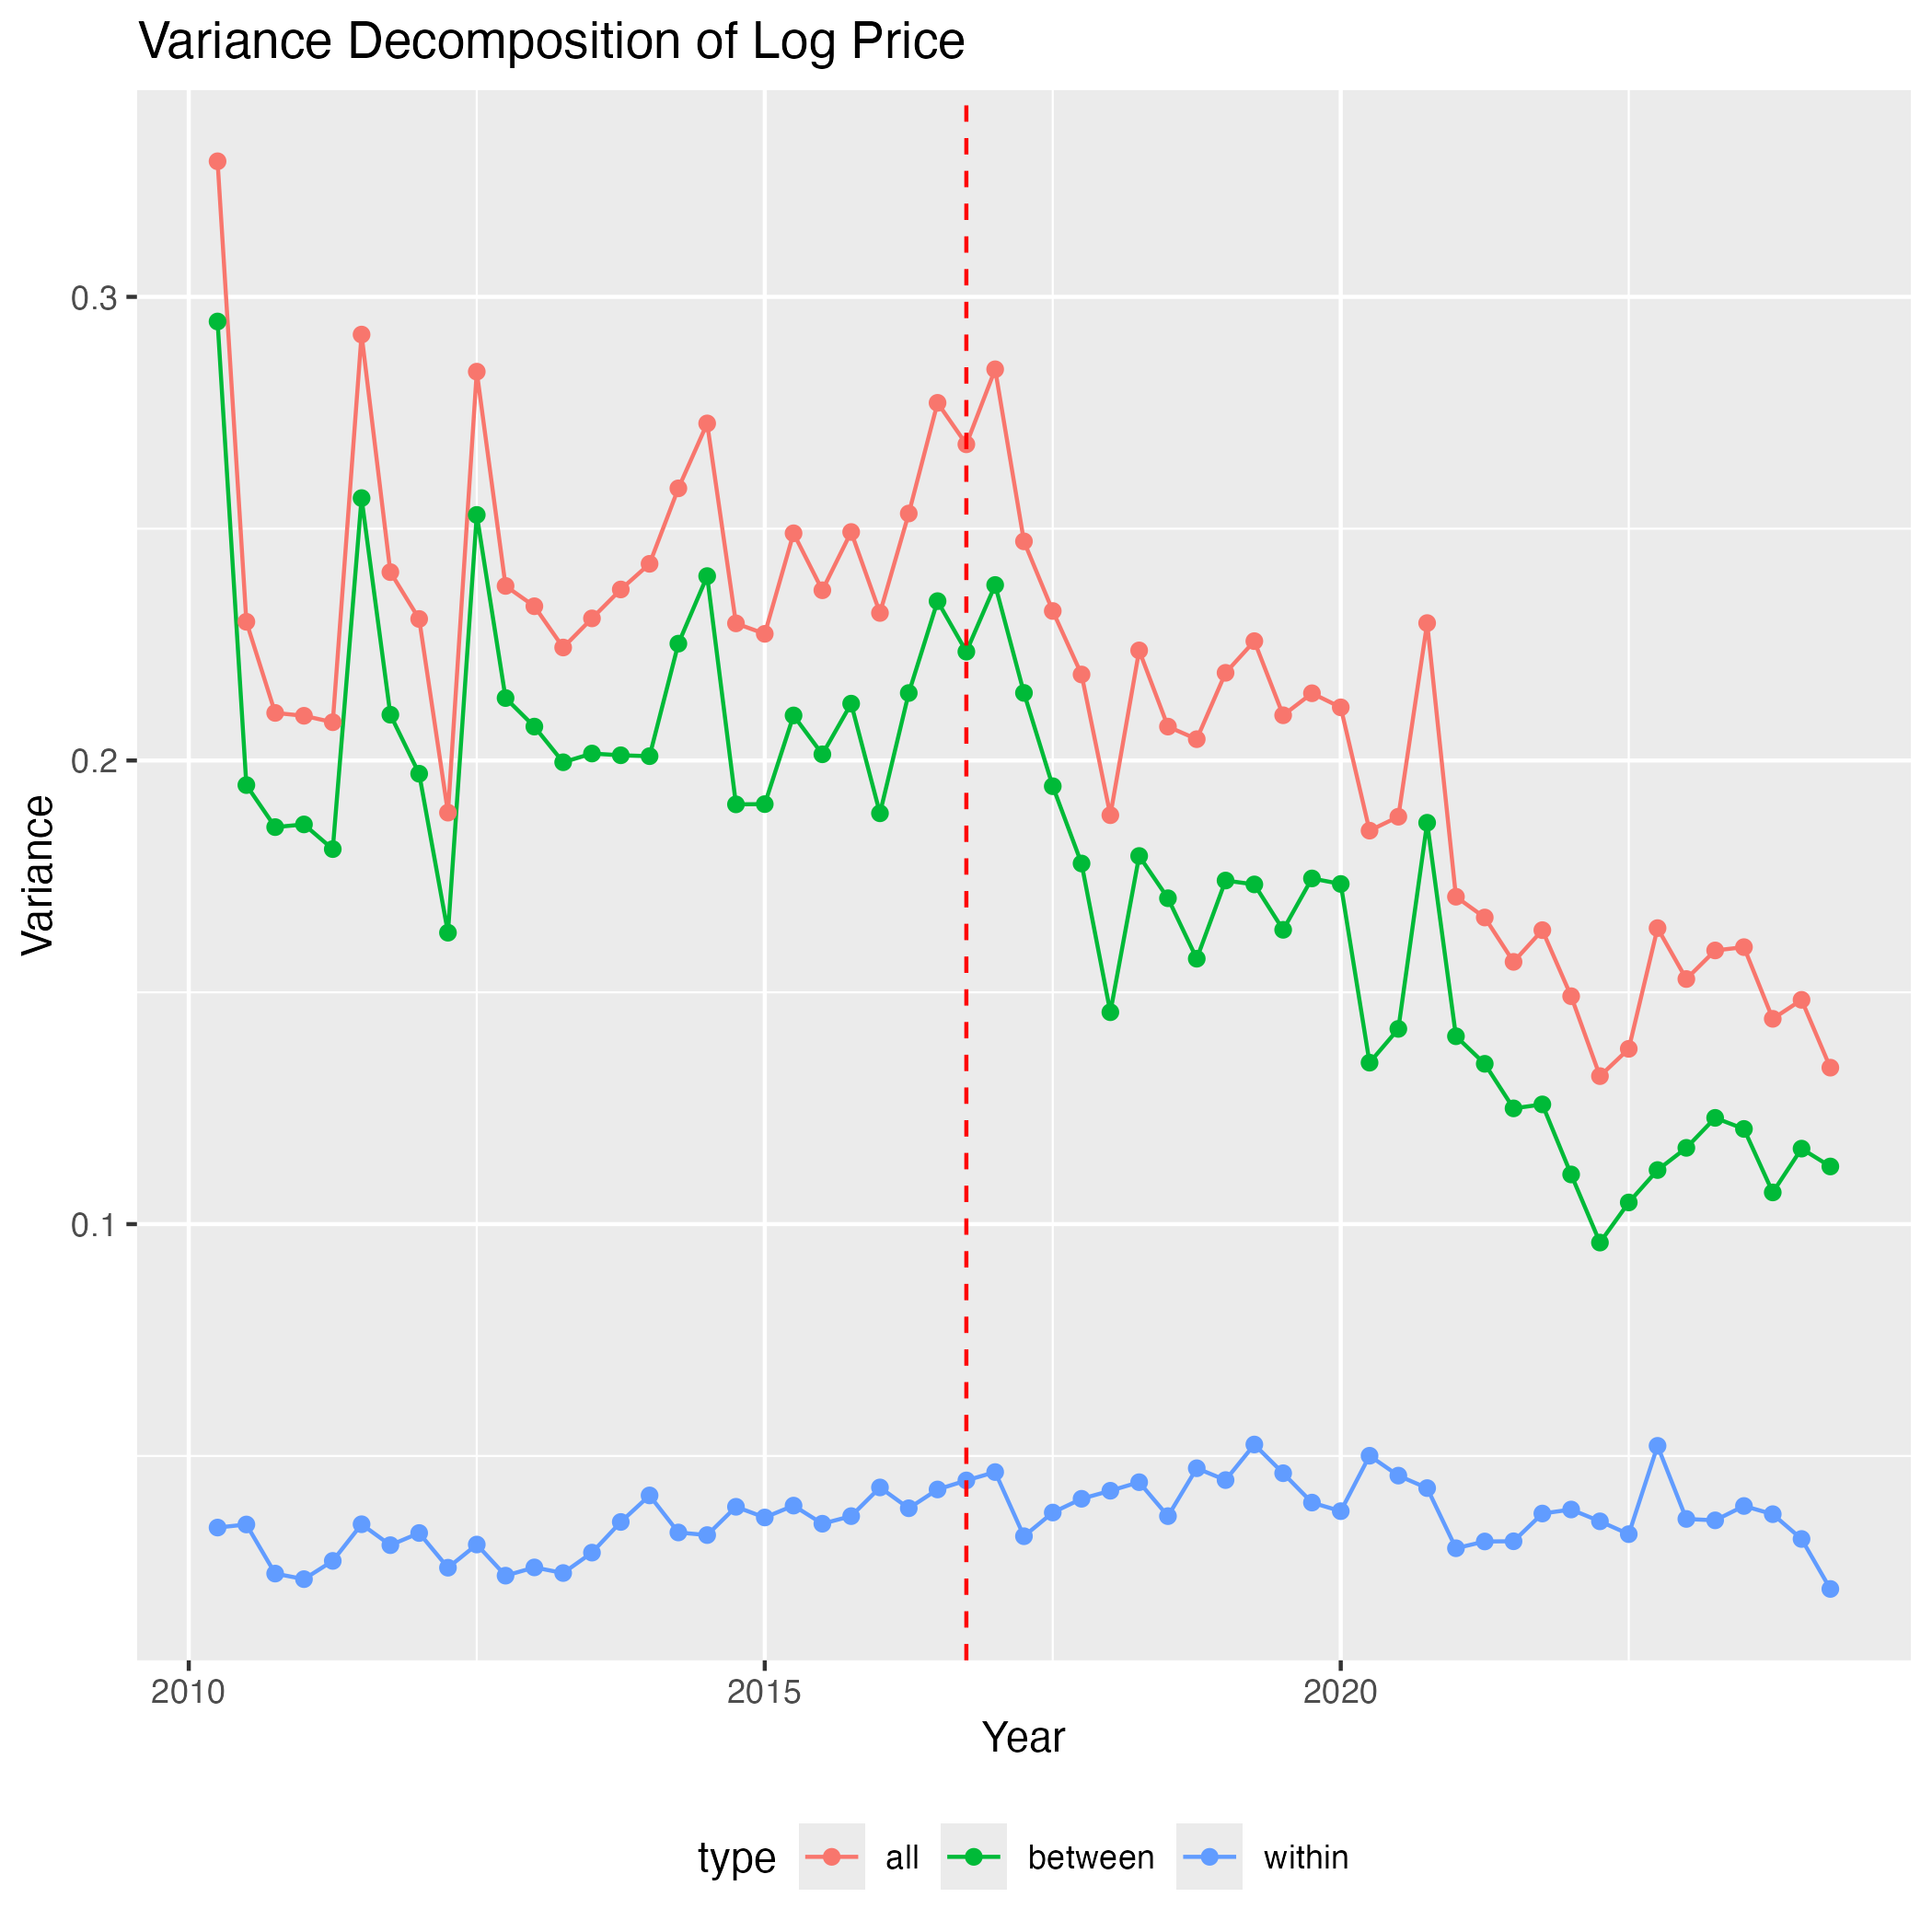
\includegraphics[width=\textwidth]{text/variance_decomposition.png}


\end{document}
